\documentclass[%
a4paper,							% alle weiteren Papierformat einstellbar
%landscape,						% Querformat
12pt,								% Schriftgröße (12pt, 11pt (Standard))
%BCOR1cm,							% Bindekorrektur, bspw. 1 cm
%DIVcalc,							% führt die Satzspiegelberechnung neu aus
%											  s. scrguide 2.4
%twoside,							% Doppelseiten
%twocolumn,						% zweispaltiger Satz
%halfparskip*,				% Absatzformatierung s. scrguide 3.1
parskip=half,
%headsepline,					% Trennline zum Seitenkopf	
%footsepline,					% Trennline zum Seitenfuß
%titlepage,						% Titelei auf eigener Seite
%normalheadings,			% Überschriften etwas kleiner (smallheadings)
%idxtotoc,						% Index im Inhaltsverzeichnis
%liststotoc,					% Abb.- und Tab.verzeichnis im Inhalt
%bibtotoc,						% Literaturverzeichnis im Inhalt
%abstracton,					% Überschrift über der Zusammenfassung an	
%leqno,   						% Nummerierung von Gleichungen links
%fleqn,								% Ausgabe von Gleichungen linksbündig
%draft								% überlangen Zeilen in Ausgabe gekennzeichnet
]
{report}


%% Deutsche Anpassungen %%%%%%%%%%%%%%%%%%%%%%%%%%%%%%%%%%%%%
\usepackage[ngerman]{babel}
\usepackage[T1]{fontenc}
\usepackage[utf8]{inputenc}
\usepackage{lmodern} %Type1-Schriftart für nicht-englische Texte
\usepackage{textcomp}

%% Konstanten %%%%%%%%%%%%%%%%%%%%%%%%%%%%%%%%%%%%%
\newcommand{\course}{Labor Projekt}
\newcommand{\exercise}{RISC-V RV32I Softcore}
\newcommand{\topic}{Dokumentation}
\newcommand{\authorname}{Guillaume Fournier-Mayer}
\newcommand{\matnum}{Tinf-101922}
\newcommand{\fachsemester}{Fachsemester 7}
\newcommand{\verwaltungssemester}{Verwaltungssemester 12}


%% Packages für Grafiken & Abbildungen %%%%%%%%%%%%%%%%%%%%%%
\usepackage{graphicx}
\usepackage{eso-pic}
\usepackage{float}


%% Hyperref %%%%%%%%%%%%%%%%%%%%%%%%%%%%%%%%%%%%%%%%%%%%%%%%%
\usepackage[final, backref=false, pagebackref=false, bookmarks=true]{hyperref}

\hypersetup{ %Ä=\304; Ö=\326; Ü=\334; ä=\344; ö=\366; ü=\374; ß=\377
  pdfauthor={\authorname},
  pdftitle={\course{}: \exercise{} \topic{}},
  pdfsubject={\course{}: \exercise{} \topic{}},
  pdfproducer={MiKTeX},
  pdfview=FitV,             % Fit, FitH, FitV
  pdfstartview=FitV,        % PDF-Viewer benutzt beim Start bestimmte Seitenbreite
                            % (Fit, FitH, FitV)
  pdfpagemode=UseOutlines,  % PDF-Viewer startet ohne Inhaltsverzeichnis et.al.
                            % (FullScreen, UseOutlines, None)
  linkcolor=black,          % Für Links in der gleichen Seite
  urlcolor=blue,            % Für Links auf URL’s
  breaklinks=false,         % Links dürfen umgebrochen werden
  colorlinks=true,
  citecolor=black,          % Farbe für \cite
  citebordercolor=0 0 0,
  filebordercolor=0 0 0,
  linkbordercolor=0 0 0,
  menubordercolor=0 0 0,
  urlbordercolor=0 0 0,
  pdfhighlight=/I,
  pdfborder=0 0 0,          % keine Box um die Links!
  bookmarksnumbered=false,
  bookmarksopen=true
}

%% Geometry %%%%%%%%%%%%%%%%%%%%%%%%%%%%%%%%%%%%%%%%%%%%%%%%%
\usepackage[a4paper]{geometry}
\geometry{includeheadfoot, headheight = 17mm, textwidth = 16cm, textheight = 23cm}

%% Subfigure %%%%%%%%%%%%%%%%%%%%%%%%%%%%%%%%%%%%%%%%%%%%%%%%%
\usepackage{subfigure}

%% Listigs %%%%%%%%%%%%%%%%%%%%%%%%%%%%%%%%%%%%%%%%%%%%%%%%%%
\usepackage{xcolor}
\definecolor{keyword}{RGB}{0, 127, 173}
\definecolor{functions}{RGB}{230, 128, 115}
\definecolor{comment}{RGB}{0, 150, 30}


\usepackage{listings}
\lstdefinelanguage{VHDL}{
   keywords=[1]{
     library,use,all,entity,is,port,in,out,end,architecture,of,
     begin,and,others,if,elsif,process,then,downto,to,case,when
   },
   morekeywords=[2]{
     to_integer,signed,unsigned,std_logic_vector,std_logic,rising_edge,falling_edge
   },
   morecomment=[l]--
}
\lstdefinestyle{vhdl}{
   language     = VHDL,
   basicstyle   = \ttfamily,
   keywordstyle = [1]\color{keyword}\bfseries,
   keywordstyle = [2]\color{functions}\bfseries,
   commentstyle = \color{comment},
   backgroundcolor=\color[gray]{0.9},
   numbers=left,
   stepnumber=1,
   showstringspaces=false,
   breaklines=true,
   columns=fullflexible,
   frame=single,
}

\lstset{
	language=C,
  basicstyle=\ttfamily,
  commentstyle = \color{comment},
  keywordstyle=[1]\color{keyword}\bfseries,
  backgroundcolor=\color[gray]{0.9},
  numbers=left,
  stepnumber=1,
  showstringspaces=false,
  breaklines=true,
  columns=fullflexible,
  frame=single,
}
 
%% TABLE %%%%%%%%%%%%%%%%%%%%%%%%%%%%%%%%%%%%%%%%%%%%%%%%%%%
\usepackage{longtable}

%% Header %%%%%%%%%%%%%%%%%%%%%%%%%%%%%%%%%%%%%%%%%%%%%%%%%%%
\usepackage{fancyhdr}
\pagestyle{fancy}
\renewcommand{\headrulewidth}{0.3pt}
\renewcommand{\footrulewidth}{0.3pt}
% Beschriftung der Kopf- und Fußzeilen (alle Seiten gleich)
\fancyhead[L]{\course{}: \exercise{}}
\fancyhead[C]{}
\fancyhead[R]{
\includegraphics[height=1.5cm]{img/fhlogo.pdf}}
\fancyfoot[L]{\authorname{} - \matnum}
\fancyfoot[C]{}
\fancyfoot[R]{\thepage}


%% Zitate %%%%%%%%%%%%%%%%%%%%%%%%%%%%%%%%%%%%%%%%%%%%%%%%%%%%%
\usepackage[backend=biber,style=alphabetic,]{biblatex}
\addbibresource{literatur.bib}

%% Formeln %%%%%%%%%%%%%%%%%%%%%%%%%%%%%%%%%%%%%%%%%%%%%%%%%%%%%
\usepackage{amsmath}

\begin{document}
\AddToShipoutPicture{
\includegraphics{img/Deckblatt.pdf}}
\begin{titlepage}

  \centering 
  { \Huge $ $ \\ }
  \vspace{5cm}
	{ \Huge
  	\course{}\\
  	\vspace{1cm}
  	\LARGE
    \exercise{}\\
    \topic{}\\}
  \vspace{8cm}
  \authorname\\
  \vspace{1cm}
  Wedel, den \today{}

\end{titlepage}
\ClearShipoutPicture
\tableofcontents
\newpage
\setcounter{page}{1}
\part{Benutzerhandbuch}
    \section{Ablaufbedingungen}
    Um den Mikrocontroller in Betrieb zu nehmen wird folgeden Soft- und Hardware benötigt.
   

    \subsection{Software}
        Als Betriebsystem wird ein Linux Betriebsystem benötigt.
        \begin{center}
            \begin{longtable}{| l | l | l |}
                \hline
                    Software & Version & Quelle \\
                \hline
                    Quartus Prime Lite & 20.1.1 & \href{https://fpgasoftware.intel.com/?edition=lite}{Intel}\\
                \hline
                    Arrow USB Programmer & 2.4.1-1 & \href{https://wiki.trenz-electronic.de/display/PD/Arrow+USB+Programmer#ArrowUSBProgrammer-DownloadSetupFiles}{Trenz Electronics}\\
                \hline
                    RISC-V GCC Toolchain & 9.2.0 & \href{https://github.com/riscv/riscv-gnu-toolchain}{RISC-V Organisation}\\
                \hline
                \caption{Benötigte Software für Inbetriebnahme}
            \end{longtable}
        \end{center}

    \subsection{Hardware}
        \begin{center}
            \begin{longtable}{| l | l | l |}
                \hline
                    Hardware & Version & Quelle \\
                \hline
                    TEI0003 - CYC1000 & 0.2 & \href{https://wiki.trenz-electronic.de/display/PD/TEI0003+Getting+Started}{Trenz Electorincs}\\
                \hline
                    Micro-USB-Kabel & 2.0 & \\
                \hline
                \caption{Benötigte Hardware für Inbetriebnahme}
            \end{longtable}
        \end{center}
    \chapter{Bedienungsanleitung}

    \section{Öffnen des Projektes}
        Zunächst wird \textit{Quartus Prime Lite} gestartet.
        Sobald das Hauptfenster geöffnet wurde kann über den Menüpunkt \textit{File}
        der Untermenüpunkt \textit{Open Project}, wie in Abbildung \ref{fig:quartus_open_project} gezeigt,
        geklickt werden. Daraufhin öffnet sich ein Dateibrowser (Abbildung \ref{fig:quartus_select_project})
        durch den das Projekt ausgewählt werden kann.
        Der relative Pfad des Projektes im Repository ist dabei \textit{RiscV-i32/CPU/Design/RiscV.qpf}
        
        \begin{figure}[H]
            \centering
            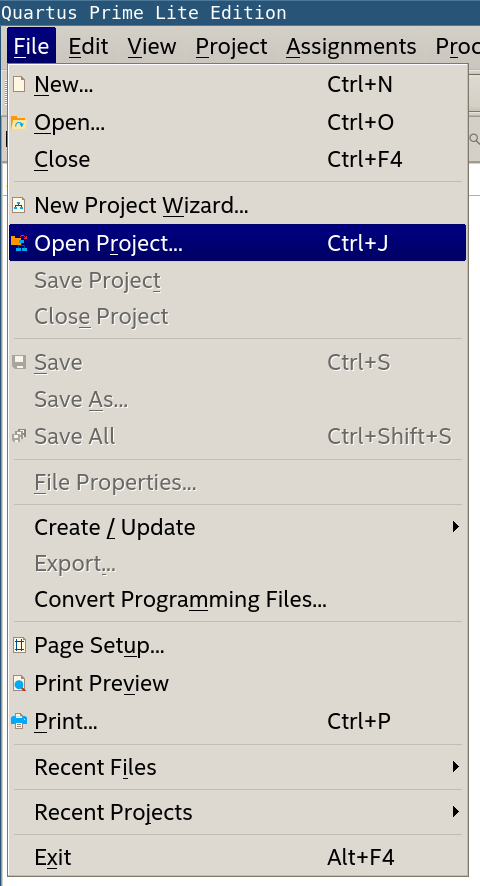
\includegraphics[scale=0.6]{img/quartus_open_project.png}
            \caption{Öffnen des Projektes in Quartus}
            \label{fig:quartus_open_project}
        \end{figure}

        \begin{figure}[H]
            \centering
            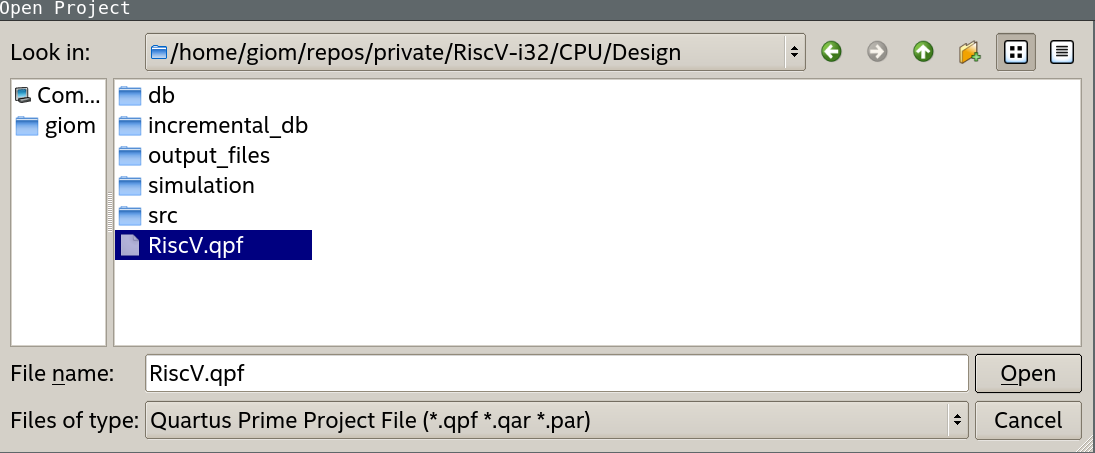
\includegraphics[scale=0.6]{img/quartus_select_project.png}
            \caption{Öffnen des Projektes in Quartus}
            \label{fig:quartus_select_project}
        \end{figure}


    \section{Bauen des Projektes}
        Sobald sich das Projekt erfolgreich geöffnet hat, kann das Bauen über einen Klick
        auf das \textit{Play}-Symbol (Abbildung \ref{fig:quartus_play}) gestartet werden. Das eigentliche Bauen kann, je nach
        Leistung des Rechners mehrere Minuten dauern. Dabei wird der Status im unteren
        Fensterdrittel angezeigt. War das Bauen erfolgreich wird die Meldung
        \textit{Quartus Prime Full Compilation was successful} (Abbildung \ref{fig:quartus_build_sucessful})
        angezeigt.

        \begin{figure}[H]
            \centering
            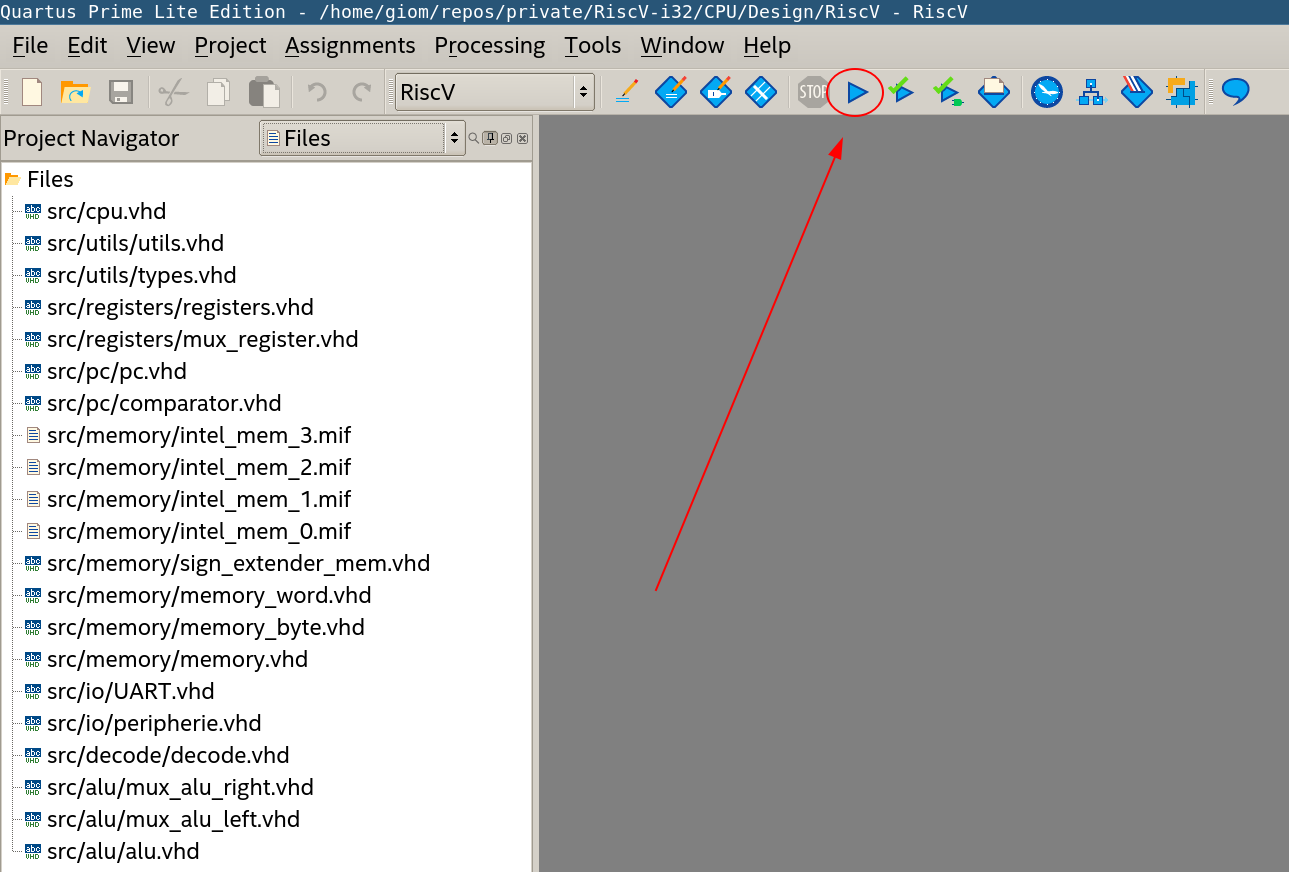
\includegraphics[scale=0.6]{img/quartus_build.png}
            \caption{Bauen des Projektes in Quartus}
            \label{fig:quartus_play}
        \end{figure}

        \begin{figure}[H]
            \centering
            
\includegraphics[scale=0.6]{img/quartus_build_sucessfull.png}
            \caption{Erfolgreiches Bauen des Projektes in Quartus}
            \label{fig:quartus_build_sucessful}
        \end{figure}


    \section{Flashen des FPGAs}

    Zunächst muss das FPGA-Board über USB angeschlossen werden. Zusätzlich muss der Treiber schon installiert sein.
    Ist dies der Fall kann über den Menüpunkt \textit{Tools} der Untermenüpunkt \textit{Programmer}
    ausgewählt werden. (Abbildung \ref{fig:quartus_programmer})
    Dadurch öffnet sich der Programmer (Abbildung \ref{fig:quartus_programmer_window})
    und die Hardware kann durch einen Klick auf \textit{Hardware Setup} eingerichtet werden.
    Ein weiteres Fenster öffnet sich (Abbildung \ref{fig:quartus_programmer_select_hardware}).
    Ein Doppelklick auf \textit{Arrow-USB-Blaster (1)} wählt das FPGA-Board als Ziel für den Programmer.
    Dies kann durch \textit{Currently selected Hardware (2)} bestätigt werden. Ein weiterer Klick 
    \textit{close} schließt das Fenster wieder. Nun kann über \textit{Start}
    (Abbildung \ref{fig:quartus_programmer_start}) das eigentliche Flashen beginnen.
    Eine visuelles Rückmeldung bietet hierbei der Ladebalken \textit{Progress}.
    

    \begin{figure}[H]
        \centering
        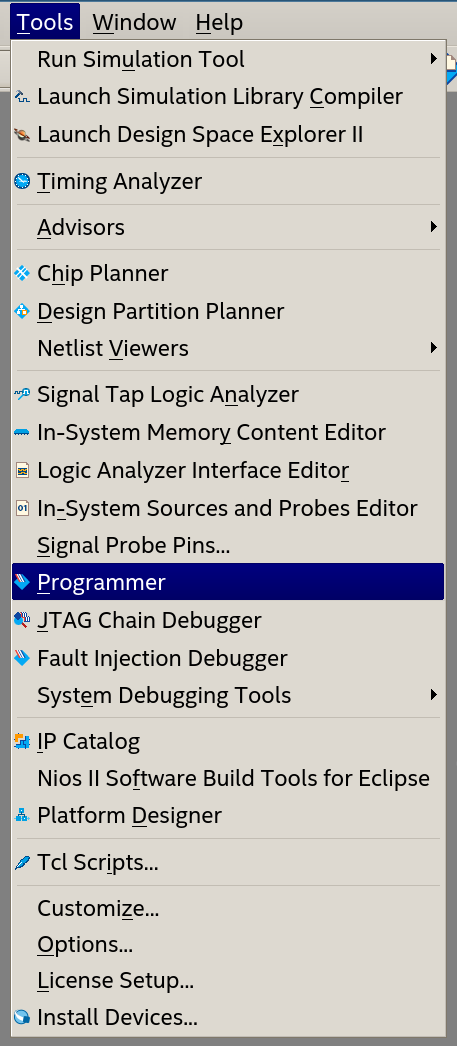
\includegraphics[scale=0.6]{img/quartus_programmer.png}
        \caption{Öffnen des Programmers in Quartus}
        \label{fig:quartus_programmer}
    \end{figure}

    \begin{figure}[H]
        \centering
        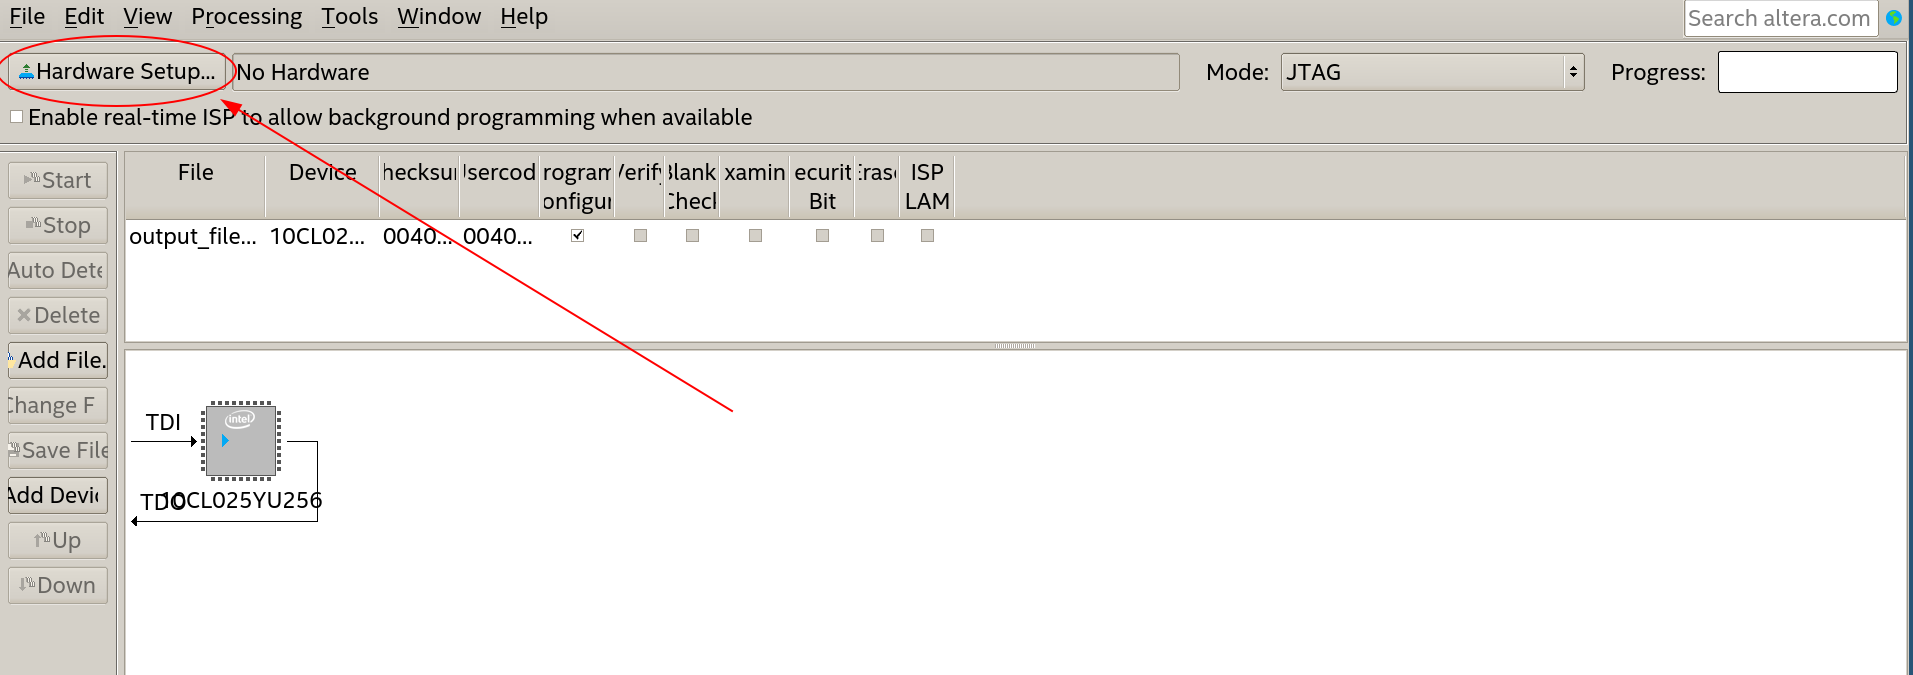
\includegraphics[scale=0.6]{img/quartus_programmer_select_hardware.png}
        \caption{Einrichten der Hardware in Quartus}
        \label{fig:quartus_programmer_window}
    \end{figure}

    \begin{figure}[H]
        \centering
        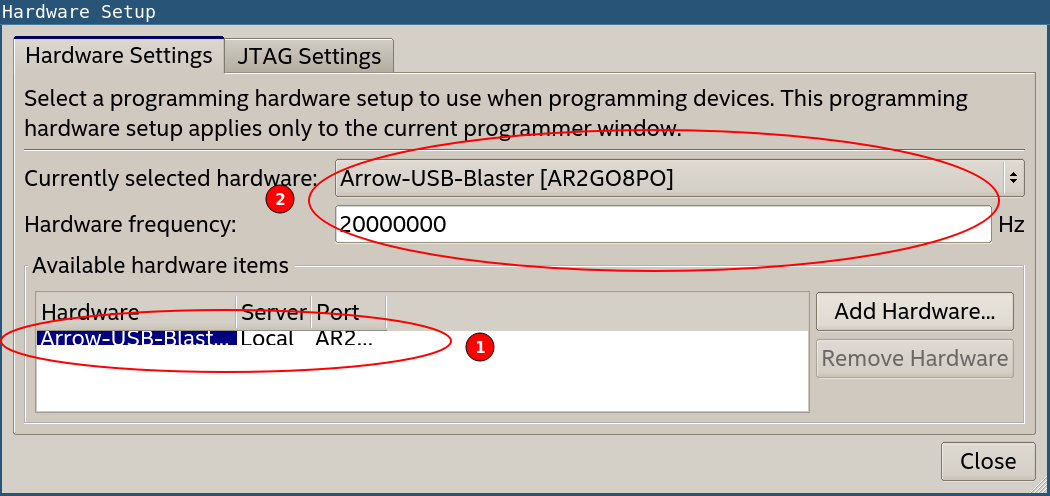
\includegraphics[scale=0.6]{img/quartus_programmer_select_hardware2.png}
        \caption{Einrichten der Hardware in Quartus}
        \label{fig:quartus_programmer_select_hardware}
    \end{figure}

    \begin{figure}[H]
        \centering
        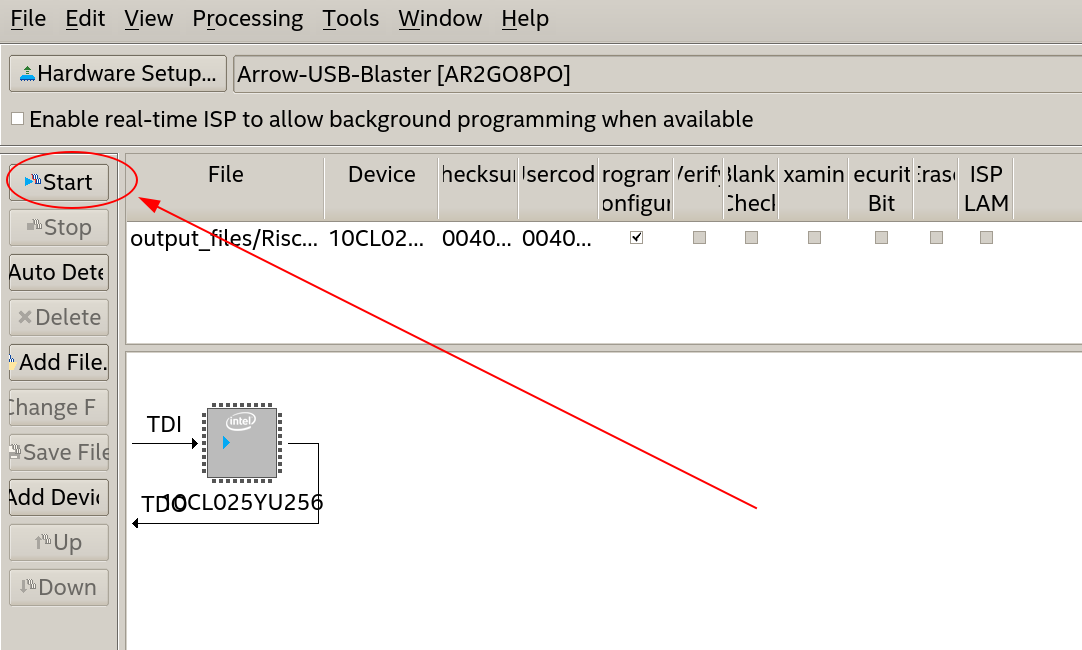
\includegraphics[scale=0.6]{img/quartus_programmer_start.png}
        \caption{Starten des Flashens des FPGAs}
        \label{fig:quartus_programmer_start}
    \end{figure}


    \section{Kompilieren des Programmcodes}
    \section{Flashen des Mikrocontrollers}




\part{Entwicklerhandbuch}

\chapter{Motivation}

    \section{RISC-V}
        \textit{RISC-V} ist eine offene und erweiterbare Befehlssatzarchitektur (ISA) die sich an dem
        \textit{RISC (Reduced Instruction Set Computer)} Designprinzip orentiert.
        Dank der freizügigen \textit{BSD-Lizenz} ist es, im Gegensatz zu bspw. der \textit{x86} ISA von \textit{Intel},
        jedem erlaubt \textit{RISC-V} Mikroprozessoren zu entwerfen, herzustellen und zu verkaufen.
        Die Lizenz erlaubt es zusätzlich den Befehlssatz nach belieben zu erweitern und somit
        optimal an eine Hardwarearchitektur anzupassen.
        In Tabelle \ref{label:riscv-base} werden die Grundbefehlssätze von RISC-V dargestellt.
        Darüber hinaus besitzt RISC-V noch zusätzliche Befehlssätze die z.B. Hardwaremultiplikation
        oder Fließkomma-Arithmetik erlauben. \cite{riscv-isa-specs}
        
        \begin{center}
            \begin{longtable}{| l | l | l |}
                \hline
                    Name & Beschreibung & Version \\
                \hline
                    RV32I & 32Bit Integer Basisbefehlssatz mit 32 Registern & 2.1 (Ratifiziert)\\
                \hline
                    RV32E & 32Bit Integer Basisbefehlssatz mit 16 Registern (Eingebettete Systeme) & 1.9 (Offen)\\
                \hline
                    RV64I & 64Bit Integer Basisbefehlssatz & 2.1 (Ratifiziert)\\
                \hline
                    RV128I & 128Bit Integer Basisbefehlssatz & 1.7 (Offen)\\
                \hline
                \caption{RISC-V Grundbefehlssätze}
                \label{label:riscv-base}
            \end{longtable}
        \end{center}

    \section{FPGA (Field Programmable Gate Array)}
        Ein FPGA, (Field Programmable Gate Array) ist ein integrierter Schaltkreis (IC) der Digitaltechnik,
        in welchen eine logische Schaltung geladen werden kann.
        Im Vergleich zu der Programmierung von Computern oder Mikrocontrollern wird die Schaltungsstruktur eines FPGAs durch eine
        Hardwarebeschreibungssprache (z.B. VHDL) beschrieben. Man spricht daher auch von der Konfiguration des FPGA.
        Ohne diese hat der Baustein keine Funktion. \cite{fpga-wiki}
        \\
        Durch einen FPGA ist es somit möglich einen \textit{RISC-V} Befehlssatz in VHDL zu formulieren und auf Hardware zu testen,
        ohne Kosten für eine Fertigung des Chips aufzubringen.


\chapter{Probelmanalyse}

    In dem Laborprojekt soll ein Softcore entwickelt werden der den \textit{RV32I} Befehlssatz implementiert.
    Dieser soll auf ein FPGA board hochgeladen werden und Programmcode ausführen können.
    Zusätzlich soll durch Simulationstests sowie durch Tests durch Programmcode die Korrektheit
    bewiesen werden.
    Die Aufgabenstellung kann in Soft- und Hardware unterteilt werden.

        \section{Software}

        \section{Hardware}\label{lab:hardware}
            Aus Hardwaresicht wird ein \textit{FPGA}-Board benötigt welches eine Möglichkeit bietet
            den in \textit{VHDL} modellierten Softcore auf das \textit{FPGA}-Board sowie Programmcode
            in den Softcore zu laden.
            \\\\
            Die Wahl fällt auf das \textit{FPGA}-Board \textit{TEI0003 TRM} von \textit{Trenz Electronic}.
            Herz des Boards ist der \textit{Cyclone 10LP 10CL025 FPGA SoC} von Intel der an einem $12 Mhz$
            Oszillator angeschlossen ist. 
            Als Speicher stehen 66 \textit{M9K}-Blöcke \cite{intel-cyc10lp-io-datasheet}[2.1 Tabelle 2] mit jeweils 8.192 Bit
            \cite{intel-cyc10lp-io-datasheet}[2.2] ($66*8192/8 = 67584B$) des \textit{Cyclone 10LP} sowie $8 MB$ des \textit{TEI0003-02} zu Verfügung.
            Abbildung \ref{fig:fpga_schematic} zeigt den schematischen Aufbau des \textit{TEI0003 TRM}.
            \begin{figure}[H]
                \centering
                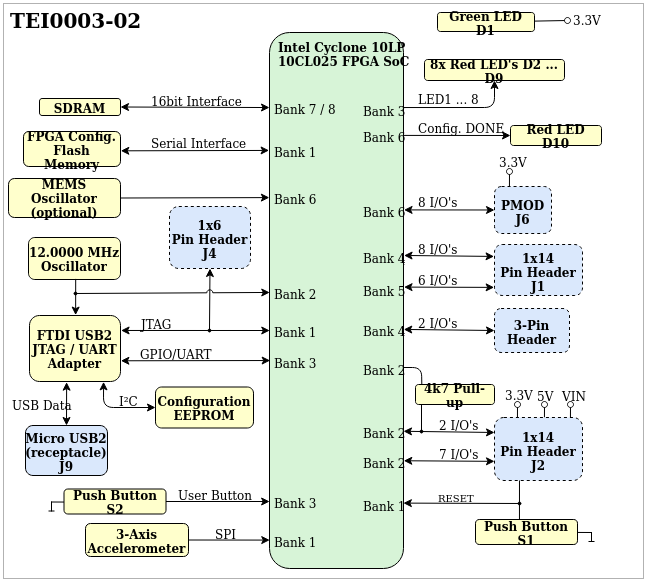
\includegraphics[scale=0.5]{img/fpga_board_schematic.png}
                \caption[Schaubild des TEI0003 TRM FPGA-Board]{Schaubild des TEI0003 TRM FPGA-Board \cite{terz} }
                \label{fig:fpga_schematic}
            \end{figure}

            \begin{figure}[H]
                \centering
                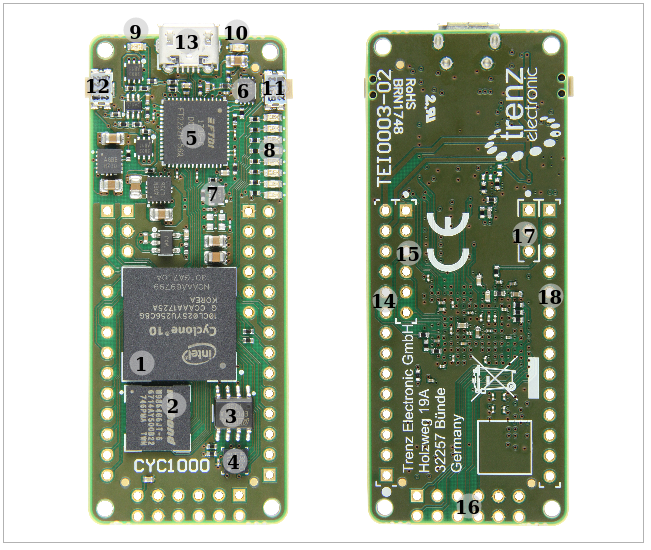
\includegraphics[scale=0.5]{img/fpga_board_layout.png}
                \caption[Platine des TEI0003 TRM FPGA-Board]{Platine des TEI0003 TRM FPGA-Board \cite{terz} }
                \label{fig:fpga_layout}
            \end{figure}

            \begin{enumerate}
                \item Intel Cyclone 10LP 10CL025 FPGA SoC, U1
                \item 8 Mbyte SDRAM 166MHz, U2
                \item 2 MByte serial configuration memory, U5
                \item ST Microelectronics LIS3DH 3-axis accelerometer, U4
                \item FTDI USB2 to JTAG/UART adapter, U3
                \item Configuration EEPROM for FTDI chip, U9
                \item 12.0000 MHz oscillator, U7
                \item 8x red user LEDs, D2 ... D9
                \item Red LED (Conf. DONE), D10
                \item Green LED (indicating supply voltage), D1
                \item Push button (user), S2
                \item Push button (reset), S1
                \item Micro USB2 B socket (receptacle), J9
                \item 1x14 pin header (2.54mm pitch), J2
                \item 1x6 pin header (2.54mm pitch), J4
                \item 2x6 Pmod connector, J6
                \item 3-pin header (2.54mm pitch), J3
                \item 1x14 pin header (2.54mm pitch), J1
            \end{enumerate}



    \section{RV32I Befehlssatz}
        Der \textit{RV32I} ist eine \textit{Load and Store} Architektur und kann somit nur mit
        Lade- bzw. Speicherbefehlen auf den Speicher zugreifen.
        Der Prozessor arbeitet nur auf den 32 Registern die zuvor mit Daten aus dem Speicher geladen werden müssen.
        Dabei bietet \textit{RV32I}, 32 Bit weite Register und kann nur Integerarithmetik in Hardware ausführen.
        \\
        Dieser Befehlssatz bietet die Basis für alle \textit{RISC-V} Befehlssätze,
        da jede Erweiterung zumindest diesen implementieren muss.
        Für den zu entwickelnden Softcore wurde somit der unprivilegierte \textit{RV32I} Befehlssatz gewählt.
        Außer acht gelassen wurden dabei die \textit{FENCE} und \textit{EBREAK} Befehle, da diese für
        den aktuellen gebrauch des Softcores nicht benötigt werden.
        \\
        Tablle \ref{tab:rv32i-types} zeigt die verschiedenen Typen des \textit{RV32I} Befehlssatzes.
        

        \begin{center}
            \begin{longtable}{| c | c | c | c | c | c | c |}
                \hline
                   Typ & 31-25 & 24-20 & 19-15 & 14-12 & 11-7 & 6-0 \\
                \hline
                    R-Type & funct7 & rs2 & rs1 & funct3 & rd & opcode \\
                \hline
                    I-Type & \multicolumn{2}{c |}{imm[11:0]} & rs1 & funct3 & rd & opcode \\
                \hline
                    S-Type & imm[11:5] & rs2 & rs1 & funct3 & imm[4:0] & opcode \\
                \hline
                    B-Type & imm[12|10:5] & rs2 & rs1 & funct3 & imm[4:1|11] & opcode \\
                \hline
                    U-Type & \multicolumn{4}{c |}{imm[31:12]} & rd & opcode \\
                \hline
                    J-Type & \multicolumn{4}{c |}{imm[20|10:1|11|19:12]} & rd & opcode \\
                \hline
                \caption[RV32I Befehlssatztypen]{RV32I Befehlssatztypen \cite{riscv-isa-specs}}
                \label{tab:rv32i-types}
            \end{longtable}
        \end{center}
        \begin{description}
            \item[R-Type] sind arithmetische und logische Befehle
            \item[I-Type] sind Immediate-, Lade- sowie relative Sprungbefehle
            \item[S-Type] sind Speicherbefehle
            \item[B-Type] sind Branchbefehle
            \item[J-Type] sind absolute Sprungbefehle
        \end{description}

    \section{Execution environment interface (EEI)}\label{lab:eei}
        Die \textit{Execution environment interface (EEI)} stellt eine Schnittstelle zur Laufzeitumgebung
        dar und definiert Initialzustände aber auch Attribute die z.B. den Speicher betreffen \cite{riscv-isa-specs}[1.2].
        Der Befehlssatz lässt viel Spielraum zu, sodass viele Werte frei gewählt werden können.
        Da der Softcore von Grund auf entwickelt wird, können viele Parameter so gewählt werden, dass sie zur Architektur passen.


    \section{Softcore Design}

        \subsection{Mikroarchitektur}
                \subsubsection{Von-Neumann-Architektur (VNA)}
                    Die nach \textit{John von Neumann} benante Mikroarchitektur \textit{Von-Neumann-Architektur (VNA)}
                    bietet eine Grundlage für die Arbeitsweise der meisten heute bekannten Computer.
                    Dabei ist charakteristisch, dass die Daten sowie das Programm im selben Speicher abgelegt sind und
                    der Zugriff auf diese nur über den selben Bus stattfindet (Abbildung \ref{fig:vonneumann}).
                    Dies hat den Vorteil, dass \textit{Race Conditions} sowie Daten-Inkohärenzen ausgeschlossen werden können.
                    Ein wesentlicher nachteil dieses Ansatzes ist der sogenante \textit{Von-Neumann-Flaschenhals}.
                    Dieser entsteht dadurch, dass die Instruktionen nicht zur gleichen Zeit gelesen,
                    wie Daten geschrieben bzw. gelesen werden können. Wenn bspw. ein Ladebefehl aus dem Programmspeicher
                    geladen wird, beinhaltet dieser die Adresse aus der die eigentlichen Daten ausgelesen werden sollen.
                    Nun kann der Adressbus aber nicht zur gleichen Zeit die Instruktion sowie die Daten ansprechen.
                    Das auslesen der Daten erfolgt somit erst im nächsten Taktzyklus. Dadurch werden für
                    die Lade- und Speicheroperationen immer zwei Zyklen verwendet, welches sich
                    negativ auf die Performance auswirkt.
                    Da es aus sicht der Speichers keinen Unterschied zwischen Instruktion und Daten gibt,
                    könnten theoretisch Daten als Instruktionen ausgelesen werden und könnte von Schadcode ausgenutzt werden.\\
                    Ein \textit{Von-Neumann-Rechner} kann in folgeden Komponenten unterteilt werden.

                    \begin{description}
                        \item[ALU (Arithmetic Logic Unit)] Das Rechenwerk führt arithmetische Operationen sowie logische Verknüpfungen durch. 
                        \item[Control Unit] Das Steuerwerk decodiert die Befehle des Programmes,
                        setzt die entsprechenden Steuerleitungen und regelt die Befehlsabfolge.
                        \item[Bus] Das Bussystem (Steuerbus, Adressbus und Datenbus) ist für die Kommunikation zwischen den einzelnen
                        Komponenten verantwortlich.
                        \item[Memory] Der Speicher, speichert das eigentliche Programm sowie die Daten.
                        \item[IO] Das Ein- bzw Ausgabewerk steuert die Ein bzw. Ausgabedaten die zum Anwender sowie zu anderen Systemen führen.
                    \end{description}
                    \begin{figure}[H]
                        \centering
                        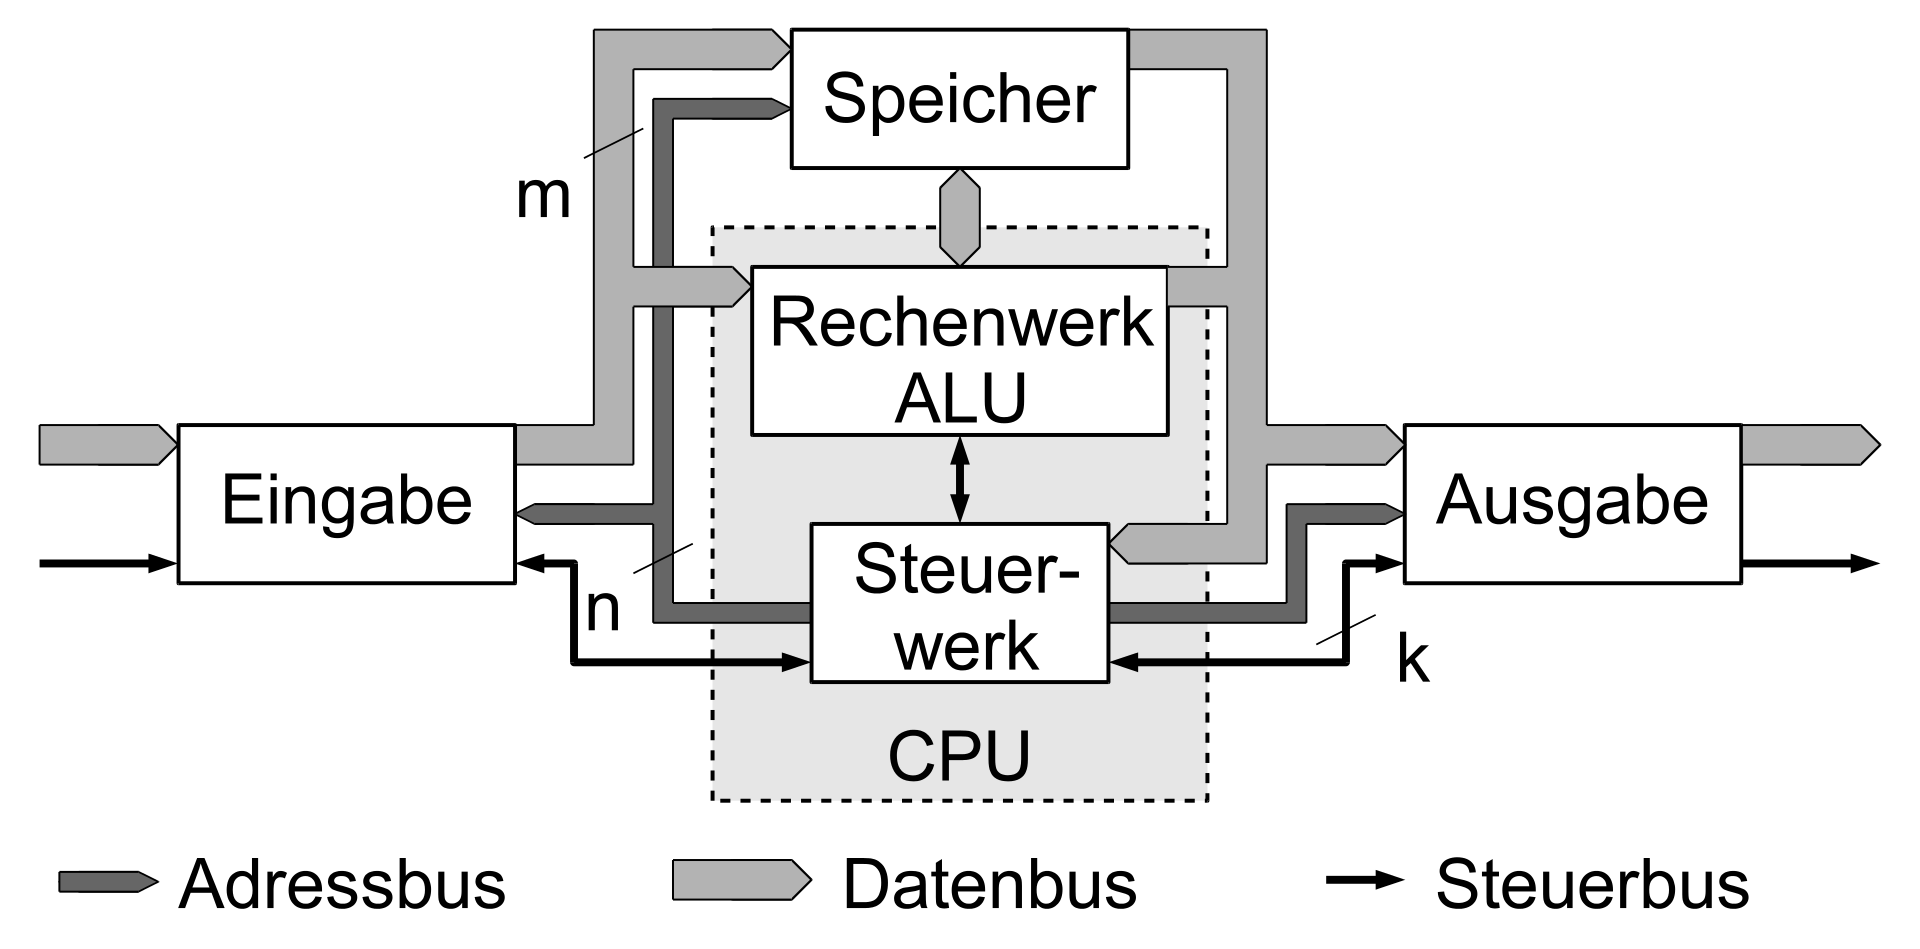
\includegraphics[scale=0.2]{img/vonneumann.png}
                        \caption[Von-Neumann-Architektur]{Von-Neumann-Architektur \cite{von-neumann-architektur}}
                        \label{fig:vonneumann}
                    \end{figure}

                \subsubsection{Harvard-Architektur}\label{lab:havard}
                    Eine weitere verbreitete Architektur ist die \textit{Harvard-Architektur}.
                    Grundlegen unterscheidet sich diese zur \textit{Von-Neumann-Architektur}
                    nur in ihrem Speicher und dem Bus. Die \textit{Harvard-Architektur} verfolgt den Ansatz,
                    Instruktionen und Daten physikalisch strikt voneinander zu trennen.
                    Dabei werden zwei separate Speicher mit eigenem Adress- sowie Datenbus verwendet.
                    Dies hat, im gegensatz zur \textit{Von-Neumann-Architektur}, den Vorteil, dass Instruktionen
                    und Daten in einem Taktzyklus gelesen bzw. geschrieben werden können. Hauptnachteil ist jedoch,
                    dass es zu Speicherfragmentierung kommt, da weder nicht genutzter Programmspeicher als Datenspeicher
                    sowie umgekehrt, genutzt werden kann.
                    \\\\
                    Für den zu entwickelnden Softcore wird eine \textit{modifizierte Harvard-Architektur} verwendet die,
                    die Vorteile der beiden oben genanten Architekturen vereint. Um die Speicherfragmentierung zu eliminieren, 
                    wird wie bei der \textit{Von-Neumann-Architektur} nur ein Speicher verwendet.
                    Jedoch werden wie bei der \textit{Harvard-Architektur} zwei Bussysteme (Instruktionsbus und Datenbus)
                    implementiert. 

        \subsection{Befehlsverarbeitung}

            \subsubsection{Von-Neumann-Zyklus}
                Die Phasen der Befehlsverarbeitung werden als \textit{Von-Neumann-Zyklus}
                bezeichnet und bestehen aus folgenden fünf Teilschritten.
                Jede Phase benötigt unterschiedlich viel Zeit um sie zu durchlaufen.
                Dabei ist zu beachten, dass nicht jede Instruktion alle Phasen durchlaufen muss.
                Eine absoluter Sprung z.B. ist schneller abgearbeitet als eine arithmetische
                Operation die zunächst die Operanden aus den Registern laden,
                verarbeiten und anschließend zurück in die Register schreiben muss.
            
                \begin{description}
                    \item[Fetch] Der Befehl wird aus dem Speicher geladen.
                    \item[Decode] Der Befehl wird dekodiert und die Steuerleitungen werden gesetzt.
                    \item[Fetch Operands] Die Operanden für die ALU werden geladen 
                    \item[Execute] Das Rechenwerk verarbeitet die Operanden
                    \item[Writeback] Das Ergebnis wird in den Speicher zurück geschrieben
                \end{description}


            \subsubsection{Cycles per Instruction (CPI)}
                \textit{Cycles per Instruction (CPI)} ist ein Maß zur Beurteilung der Performanz eines Prozessors
                und sagt aus wie viele Taktzyklen benötigt werden um eine Instruktion abzuarbeiten.
                Je kleiner der CPI Wert ist desto performanter kann ein Prozessor eingeschätzt werden.
                \begin{equation}
                    CPI = \frac{Taktzyklen}{Instruktion}
                \end{equation}
                Dabei wird ein Prozessor mit einem CPI Wert größer als eins ($CPI > 1$) als subskalar,
                mit einem Wert gleich eins ($CPI = 1$) als skalar und mit einem Wert kleiner als eins
                ($CPI < 1$) als superskalarer Prozessor bezeichnet.
   

            \subsubsection{Ein-Zyklus-Prozessor}
                Als Ein-Zyklus-Prozessor wird ein Prozessor verstanden der alle Phasen des \textit{Von-Neumann-Zyklus}
                in einem Taktzyklus abarbeitet.
                Somit ergibt sich ein CPI-Wert von eins ($CPI = 1$) und der Prozessor kann als \textit{Skalar} bezeichnet werden.
                Die maximal Taktfrequenz bzw. die minimale Taktzeit ist dabei direkt abhängig von der Signallaufzeit
                der längsten Instruktion.
                \begin{equation}
                    Taktzeit > Signallaufzeit_{Gesamtbefehl}
                \end{equation}
                Ein wesentlicher Vorteil dieser Architektur ist die einfache implementierung, da
                keine zusätzliche Logik benötigt wird.

            \subsubsection{Pipelining-Prozessor}
                Im gegensatz zum Ein-Zyklus-Prozessor steht der Pipelining-Prozessor.
                Statt eines gesamten Befehls wird während eines Taktzyklus nur jeweils eine Teilaufgabe abgearbeitet.
                Dabei können Teilaufgaben mehrerer Befehle gleichzeitig abgearbeitet werden.
                Eine Teilaufgabe kann dabei z.B. eine \textit{Von-Neumann-Phase} sein oder noch feiner Granuliert werden.
                Da eine Teilaufgaben eine kürzere Signallaufzeit aufweist als der Gesamtbefehl,
                kann die Taktzeit kürzer sein als die Signallaufzeit des Gesamtbefehls.
                \begin{equation}
                    \begin{split}
                        Taktzeit < Signallaufzeit_{Gesamtbefehl} \\
                        Taktzeit > Signallaufzeit_{Teilaufgabe}
                    \end{split}
                \end{equation}
                Die Taktzeit ist somit nur noch abhängig von der Signallaufzeit der Teilaufgabe die am längsten dauert.
                Die Teilaufgaben eines Befehls werden auch \textit{Pipeline-Stages} genant.
                Abbildung \ref{fig:pipelining} zeigt eine vierstufige Befehlspipeline und der daraus resultierende erhöhte Gesamtdurchsatz.
                Ein wesentlicher Nachteil von Pipelining sind jedoch die Konflikte \textit{(Pipeline-Hazards)}
                die dabei auftretten können. Dabei können folgende drei Konfliktarten auftretten.
    
                \begin{description}
                    \item[Ressourcenkonflikte] wenn eine Stufe der Pipeline Zugriff auf eine Ressource benötigt, die bereits von einer anderen Stufe belegt ist 
                    \item[Datenkonflikte] wenn ein Befehl, der sich in der Pipeline befindet abhängig von einem Befehl ist der weiter vorne ist.
                    \item[Kontrollflusskonflikte] wenn die Pipeline abwarten muss, ob ein bedingter Sprung ausgeführt wird oder nicht
                \end{description}
                \begin{figure}[H]
                    \centering
                    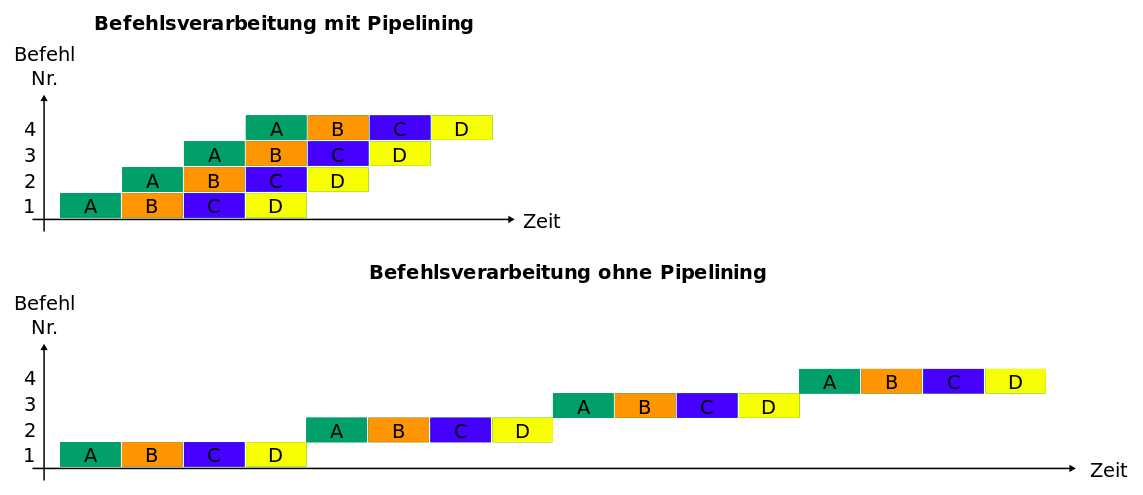
\includegraphics[scale=0.375]{img/pipelining.png}
                    \caption[Befehlsverarbeitung mit und ohne Pipelining]{Befehlsverarbeitung mit und ohne Pipelining \cite{pipelining} }
                    \label{fig:pipelining}
                \end{figure}
                \begin{description}
                    \item[A: Befehlscode laden (IF, Instruction Fetch)] 
                    \item[B: Instruktion dekodieren und Laden der Daten (ID, Instruction Decoding)] 
                    \item[C: Befehl ausführen (EX, Execution)] 
                    \item[D: Ergebnisse zurückgeben (WB, Write Back)] 
                \end{description}
                Es ist jedoch zu beachtet, dass Pipelining nur von Vorteil ist, wenn die Taktfrequenz, aufgrund der höheren Signallaufzeiten
                in einem Ein-Zyklus-Prozessor, nicht weiter erhöht werden kann.
                Da das gewählte \textit{FPGA}-Board nur mit $12 Mhz$ Taktet ist eine Pipelining-Architektur
                nicht von Vorteil für den Softcore, sodass eine Ein-Zyklus-Architektur gewählt werden kann um die Softcore zu implementieren.
                Dies hat zusätzlich den Vorteil, dass weniger Logikblöcke des \textit{FPGA's} benutzt werden.



        \subsection{Speicher}
                
            \subsubsection{Memory Wall}
                Als \textit{Memory Wall} bezeichnet man das wachsende Ungleichgewicht zwischen der Prozessor- und der Speichergeschwindigkeit.
                Bei frühen Computern war der Prozessor die langsamste Einheit des Rechners \cite{memory-wall}.
                Die Datenbereitstellungszeit stellte somit nur ein geringen Anteil an der Verarbeitungszeit dar.
                Seit den 1980 Jahren begann jedoch der Prozessor exponentiell schneller zu werden als der Speicher \cite{memory-cpu-gap}.
                Es kann davon ausgegangen werden dass jede fünfte Instruktion den Speicher beansprucht \cite{memory-wall}.
                Somit würde der Prozessor $20\%$ der Zeit auf Daten warten. Ein idealer Speicher würde so schnell wie der Prozessor sein
                und die Daten in einem Taktzyklus liefern.
                Wie Abbildung \ref{fig:memory-hierarchy} zeigt, wäre solch ein Speicher sehr teuer.
                Eine Maßnahme um der \textit{Memory Wall} entgegen zu wirken ist der einsatz von Cachespeicher direkt im Prozessor.
                \\\\
                Auf dem \textit{FPGA}-Board stehen die \textit{M9K}-Blöcke sowie \textit{SDRAM} als Speicher zu Verfügung (Siehe \ref{lab:hardware}).
                Dabei wir der \textit{SDRAM} über eine 16 Bit Interface angesprochen. Der \textit{RV32I} Befehlssatz ist jedoch 32 Bit breit.
                Dadurch werden zwei Taktzyklen benötigt um eine Instruktion aus dem Speicher zu laden und würde den Softcore ausbremsen.
                Um das Problem der \textit{Memory Wall} zu lösen werden die \textit{M9K}-Blocke des FPGA's als Speicher benutzt.
                Diese können in der Breite frei variiert werden und ermöglichen den Zugriff auf die Daten in einem Taktzyklus.
                Wesentlicher Nachteil dieser Lösung ist, dass nur \textit{67584B} Speicher für Daten und Instruktionen zu Verfügung stehen.
                
                \begin{figure}[H]
                    \centering
                    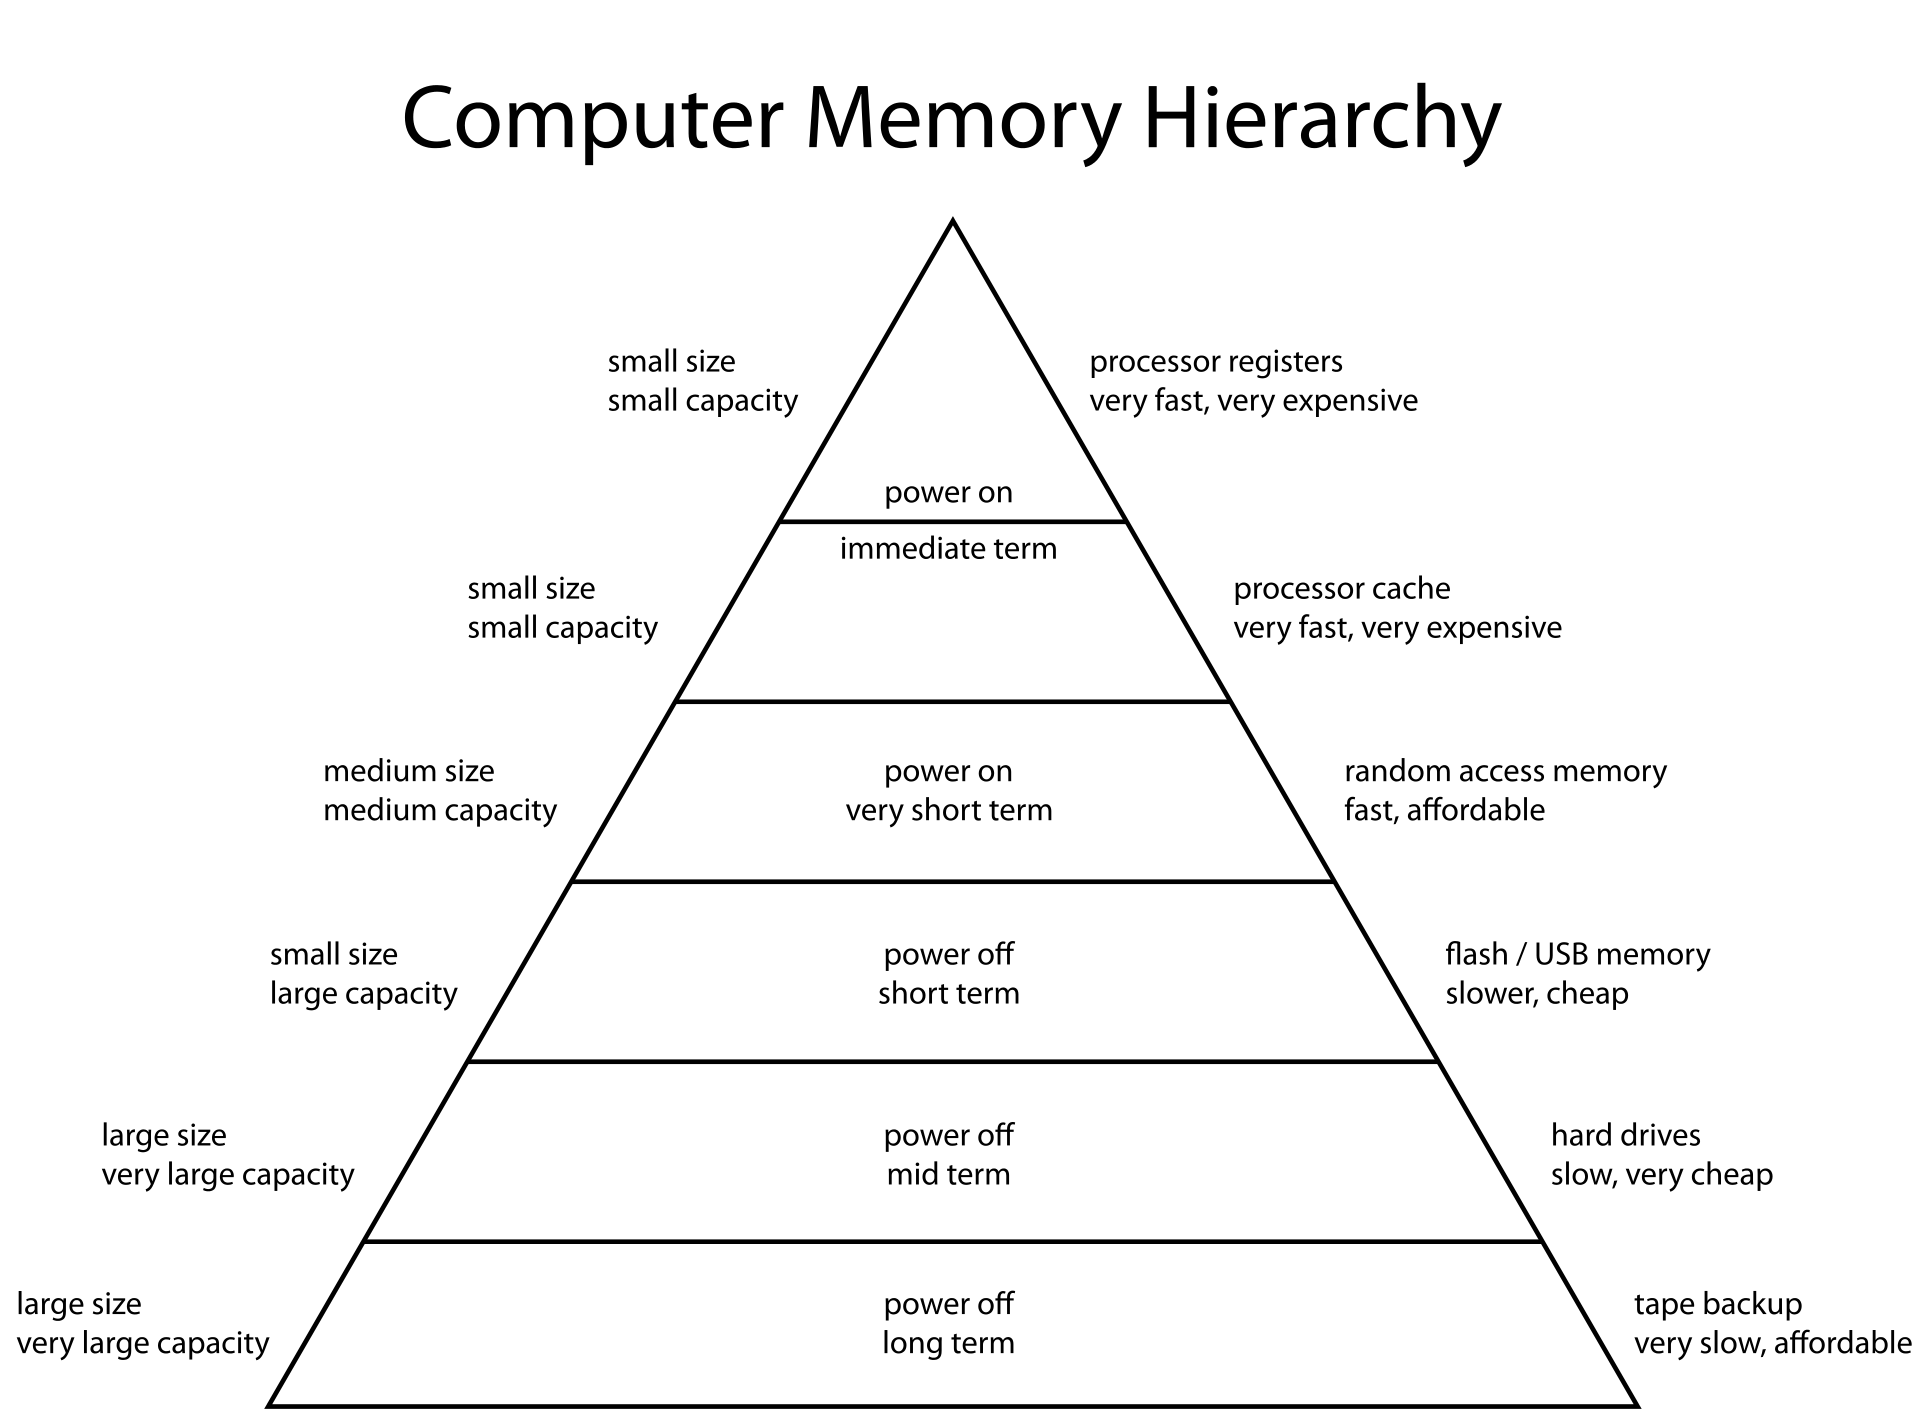
\includegraphics[scale=0.2]{img/speicherpyramide.png}
                    \caption[Speicherpyramide]{Speicherpyramide \cite{memory-hierarchy}}
                    \label{fig:memory-hierarchy}
                \end{figure}


            \subsubsection{Speicherausrichtung}\label{lab:mem-order}
                Da eine \textit{modifizierte Harvard-Architektur} gewählt wurde (Siehe \ref{lab:havard}) liegen im Speicher
                sowohl Daten als auch Instruktionen. Die Instruktionen sind hierbei in vier Byte Grenzen zu halten
                (natürliche Ausrichtung) \cite{riscv-isa-specs}[2.2].
                Der Befehlssatz lässt es jedoch der EEI (Siehe \ref{lab:eei}) überlassen, ob die Daten auch natürlich ausgerichtet liegen sollen
                \cite{riscv-isa-specs}[2.6].
                Der Vorteil von natürlich ausgerichteten Daten liegt darin, das keine zusätzliche Logik benötigt wird um Daten im Speicher
                auszulesen bzw. zu schreiben. Wesentlicher Nachteil ist die Speicherfragmentierung. Da im Worst-case 32 Bit für einen 8 Bit 
                Wert verbraucht werden. Die ungenutzten 24 Bit $(32 Bit - 8 Bit = 24 Bit)$ werden mit Nullen aufgefüllt.
                Der Einfachheit halber wird der Ansatz des natürlich ausgerichteten Speicher gewählt.

                





                
            
                
            
           
            
            

            

            



            
    
        

    

\chapter{Realisation in VHDL}

    Folgendes Kapitel gibt eine Übersicht über die implementierten Einheiten (Entitys) in VHDL.
    \begin{figure}[H]
        \centering
        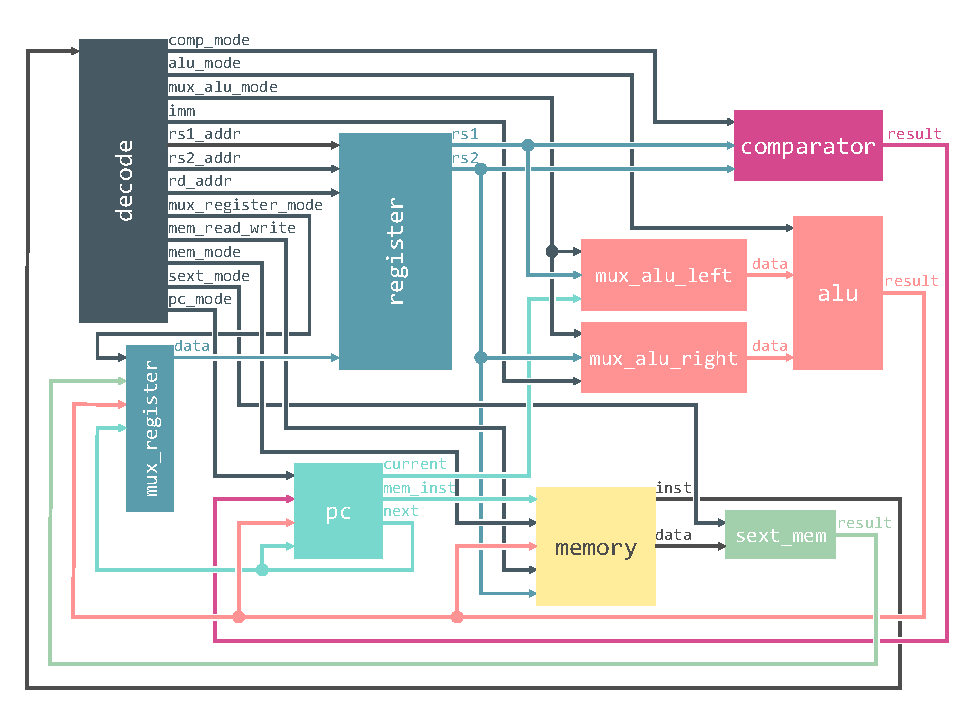
\includegraphics[scale=1]{img/OverviewCPU.pdf}
        \caption{Gesamtübersicht des Softcores}
        \label{fig:cpu_overview}
    \end{figure}


    \section{Steuerwerk}

        Die Dekodiereinheit wid im Verbund mit dem \textit{Programm Counter (PC)} (Siehe \ref{lab:pc}) auch Steuerwerk genant.

        \begin{figure}[H]
            \centering
            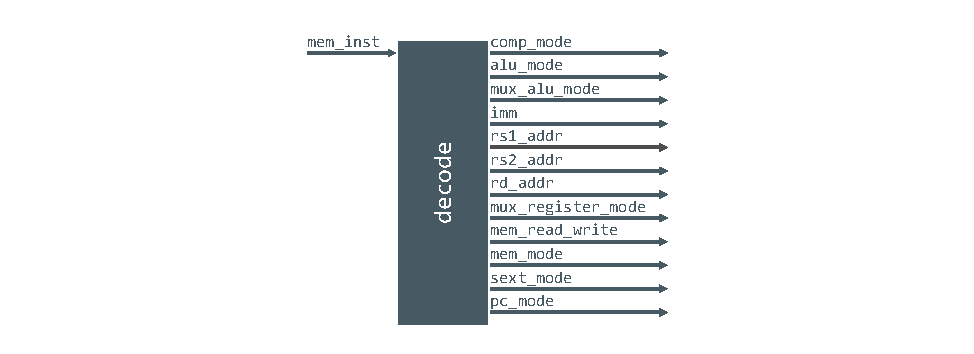
\includegraphics[scale=1]{img/block_decode.pdf}
            \caption{Dekodiereinheit}
            \label{fig:decode}
        \end{figure}

        \subsection{Dekodiereinheit}
            
            Die Dekodiereinheit ist dafür zuständig die Instruktionen aus dem Speicher zu interpretieren und die notwendigen
            Steuerleitungen zu setzen.
            Hierfür ist die Einheit direkt über den 32 Bit Instruktionbus mit dem Speicher verbunden.

        \subsection{Programm Counter (PC)}\label{lab:pc}

            \begin{figure}[H]
                \centering
                
\includegraphics[scale=1]{img/block_pc.pdf}
                \caption{Befehlszählers}
                \label{fig:pc}
            \end{figure}

            Der Befehlszähler steuert den Programmablauf und speichert in einem 32 Bit Register
            die aktuelle Adresse der Instruktion im Programspeicher.
            In jedem Taktzyklus wird die Adresse um ein Wort (32 Bit) erhöht und zeigt somit
            auf den nächsten Befehl. Dieser kann wieder von der Dekodiereinheit dekodiert werden
            und es können die Steuerleitungen gesetzt werden. Der Befehlszähler kann jedoch nicht nur
            inkrementiert sondern auch überschrieben werden.
            \newpage
            \lstinputlisting[style=vhdl,linerange={37-47},caption={Prozess des Befehlszählers}]{../../CPU/Design/src/pc/pc.vhd}

        \subsection{Branch}

            \begin{figure}[H]
                \centering
                
\includegraphics[scale=1]{img/block_comparator.pdf}
                \caption{Vergleichswerk}
                \label{fig:alu}
            \end{figure}

            Wenn eine Anweisung zur Ablaufsteuerung auf Programmebene
            ausgeführt werden soll, muss zunächst die Bedingung geprüft werden
            und dann ggfs. eine Instruktion ausgeführt werden,
            die nicht sequentiell hinter der aktuellen im Speicher liegt.
            Dies nennt man einen Zweig (englisch: Branch). Ein Zweig erfordert zusätzliche Logik in Steuerwerk 
            und wird durch eine Vergleichseinheit realisiert.
            Diese Einheit vergleicht zwei 32 Bit Daten (Links und Rechts) und liefert ein boolesches Ergebnis (ein Bit).
            Tabelle \ref{tab:comp-states} zeigt welche Vergleichsoperatoren zu Verfügung stehen.

            \begin{center}
                \begin{longtable}{| l | l | }
                    \hline
                        Zustand & Operation \\
                    \hline
                        COMP\_EQUAL & signed(links) == signed(rechts) \\
                    \hline
                        COMP\_NOT\_EQUAL & signed(links) != signed(rechts) \\
                    \hline
                        COMP\_LESS\_THEN & signed(links) < signed(rechts) \\
                    \hline
                        COMP\_GREATER\_EQUAL & signed(links) >= signed(rechts) \\
                    \hline
                        COMP\_LESS\_THEN\_U & unsigned(links) < unsigned(rechts) \\
                    \hline
                        COMP\_GREATER\_EQUAL\_U & unsigned(links) >= unsigned(rechts) \\
                    \hline
                    \caption[Zustandstabelle Vergleichswerk]{Zustandstabelle Vergleichswerk}
                    \label{tab:comp-states}
                \end{longtable}
            \end{center}
                


    \section{Register}

        \begin{figure}[H]
            \centering
            
\includegraphics[scale=1]{img/block_register.pdf}
            \caption{Registereinheit}
            \label{fig:register}
        \end{figure}


        \subsection{Registereinheit} 
            Die Registereinheit bildet 32 Register mit einer Breite von 32 Bit ab \cite{riscv-isa-specs}[2.1].
            Dabei kann in einem Taktzyklus auf zwei Register (rs1 und rs2) lesend und auf einem Register (rd) schreibend zugegriffen werden.
            Die \textit{ISA} besagt zudem, dass Register x0 immer Nullen liefern soll und nicht überschrieben werden darf \cite{riscv-isa-specs}[2.1].
            Dies wird durch eine Abfrage der Adresse im Prozess gesteuert. Falls das Zielregister, das Nullregister sein sollte werden die Werte
            nicht in das Zielregister übernommen.
            \lstinputlisting[style=vhdl,linerange={47-55},caption={Prozess der Registereinheit}]{../../CPU/Design/src/registers/registers.vhd}

        \subsection{Register Multiplexer}

            \begin{figure}[H]
                \centering
                
\includegraphics[scale=1]{img/block_mux_register.pdf}
                \caption{Register Multiplexer}
                \label{fig:register_mux}
            \end{figure}


            Die Eingangsdaten werden instruktionsabhängig augewählt und in das Zielregister (rd) geschrieben.
            Dies geschieht in einem vorgeschaltetem Multiplexer. Die Dekodiereinheit setzt dabei die notwendigen Steuerleitungen.
            Als Auswahlmöglichkeiten der Daten stehen die \textit{ALU}, der Speicher, der nächste Befehlszähler (PC + 4).
            Als gesonderte Absicherung dient der \textit{MUX\_REG\_ZERO} Zustand.
            Dieser wird standardmäßig beim initialisieren gesetzt und soll ein Überschreiben von Daten verhindern wenn z.B.
            eine unbekannte Instruktion ausgeführt werden soll.
            \lstinputlisting[style=vhdl,linerange={28-39},caption={Prozess des register Multiplexers}]{../../CPU/Design/src/registers/mux_register.vhd}

    \section{Arithmetic logic unit (ALU)}

        \begin{figure}[H]
            \centering
            
\includegraphics[scale=1]{img/block_alu.pdf}
            \caption{ALU}
            \label{fig:alu}
        \end{figure}

        \subsection{Rechenwerk}
            Die \textit{Arithmetic logic unit (ALU)} ist das Rechenwerk und berechnet arith­me­tisch sowie logische Operationen.
            Dabei werden nicht nur Register-Register Berechnungen sondern auch Immediate- sowie Sprungberechnungen
            basierend auf dem aktuellen Befehlszähler durchgeführt.
            Da der Befehlssatz nur Integer Operationen erlaubt können auch nur diese in Hardware umgesetzt werden \cite{riscv-isa-specs}[2.4].
            Ebenfalls fehlen der \textit{ISA} Multiplikation sowie Division.
            Diese können über Softwarebibliotheken mit Addition und Subtraktion durchgeführt werden,
            benötigen jedoch mehr Instruktionen, verbrauchen dadurch mehr Programmspeicher und schlagen sich somit negativ auf die Performanz aus.

        \subsection{Rechenwerk Multiplexer}

            \begin{figure}[H]
                \centering
                
\includegraphics[scale=1]{img/block_mux_alu_left.pdf}
                \caption{Linker ALU Multiplexer}
                \label{fig:alu_mux_left}
            \end{figure}

            \begin{figure}[H]
                \centering
                
\includegraphics[scale=1]{img/block_mux_alu_right.pdf}
                \caption{Rechter ALU Multiplexer}
                \label{fig:alu_mux_right}
            \end{figure}

            Die beiden Rechenwerk Multiplexer (Links und Rechts) steuern die Eingangsdaten des Rechenwerks und bestimmen somit welche Daten
            berechnet werden. Die Steuerleitungen werden dabei instruktionsabhängig in der Dekodiereinheit gesetzt.
            Beide Multiplexer teilen die selben Zustände, reagieren jedoch anders.
            Tabelle \ref{tab:alu-mux} zeigt die verschiedenen Zustände und die damit verbundenen Eingangsdaten für die \textit{ALU}.


            \begin{center}
                \begin{longtable}{| l | c | c | l |}
                    \hline
                        Zustand & Linker Operand & Rechter Operand & Berechnung \\
                    \hline
                        MUX\_ALU\_RS1\_RS2 & rs1 & rs2 & Register-Register \\
                    \hline
                        MUX\_ALU\_RS1\_IMM & rs1 & immediate &  Register-Immediate\\
                    \hline
                        MUX\_ALU\_PC\_IMM & pc & immediate & Sprung \\
                    \hline
                        MUX\_ALU\_PC\_RS2 & pc & rs2 & Sprung \\
                    \hline
                    \caption[Zustandstabelle ALU Multiplexer]{Zustandstabelle ALU Multiplexer}
                    \label{tab:alu-mux}
                \end{longtable}
            \end{center}

            \lstinputlisting[style=vhdl,linerange={26-37},caption={Prozess des linken Rechenwerk Multiplexers}]{../../CPU/Design/src/alu/mux_alu_left.vhd}
            \lstinputlisting[style=vhdl,linerange={27-38},caption={Prozess des rechten Rechenwerk Multiplexers}]{../../CPU/Design/src/alu/mux_alu_right.vhd}

    \section{Memory}\label{lab:memory}

        Durch die gewählte \textit{modifizierte Havard-Architektur} und den \textit{Ein-Zyklus-Ansatz}
        muss sicherstegestellt werden, dass in einem Taktzyklus sowohl Instruktion gelesen als auch die damit verbundenen Daten
        gelesen bzw. geschrieben werden können. Dies wird dadurch ermöglicht, dass die Instruktionen zur steigenden Taktflanke
        gelesen und die Daten zur fallenden Taktflanke gelesen bzw. geschrieben werden.
        Dies ist nur möglich, da die Taktzeit mehr als doppelt so lang ist, wie die Zeit die benötigt wird um eine Speicheroperation
        durchzuführen \cite{intel-cyc10lp-device-datasheet}[Tabelle 23].

        \begin{equation}
            \frac{1}{12Mhz} > 2\cdot\frac{1}{238Mhz}
        \end{equation}


        \begin{figure}[H]
            \centering
            
\includegraphics[scale=1]{img/Timing_Memory.pdf}
            \caption{Taktflanken am Speicher}
            \label{fig:timing_memory}
        \end{figure}

         \begin{enumerate}
             \item Neue Instruktionsadresse muss bereits anliegen
             \item Instruktion wird aus Speicher gelesen / Steuerwerk setzt Kontrollsignale
             \item Instruktion wird ausgeführt / Adresse für Daten wird berechnet.
             \item Daten werden an berechneter Adresse geschrieben bzw. gelesen
             \item Gelesen Daten werden durch ALU verrechnet und in Zielregister geschrieben. / Daten werden aus Register in Speicher geschrieben
         \end{enumerate}

            
        \subsection{Byte-Adressierung}
            Auch wenn die Speicherausrichtung natürlich ist (Siehe \ref{lab:mem-order}), fordert der Befehlssatz eine Byte-Adressierung,
            sodass auf einzelne Bytes in einem Wort zugegriffen werden kann. Leider erlauben das die \textit{M9K} Speicherblöcke nicht.
            Aus diesem Grund wurden vier Speicherpartitionen erstellt die jeweils ein Viertel des gesamten Speichers ausmachen.
            Soll nur ein einzelnes Byte gelesen bzw. geschrieben werden, wird nur eine Speicherpartition adressiert.
            Bei einem \textit{half-Word} werden hingegen zwei Partitionen ausgelesen. Dabei wird sichergestellt,
            dass nicht über die natürliche Ausrichtung hinweg adressiert werden kann.
            Eine Speicherpartition wird durch \textit{memory\_byte.vhd} repräsentiert und wird durch die \textit{Megafunction} erstellt.
            Somit wird gewährleistet, dass die \textit{M9K}-Blöcke des \textit{FPGA's} benutzt werden.
            In \textit{memory\_word.vhd} wird die Logik definiert, die zuständig ist um bei jeweiliger Adresse die 
            richtige Speicherpartition zu adressieren.
            Für Instruktionen und Daten stehen insgesamt 65535 Bytes zu Verfügung.

        \subsection{Initialisierung}\label{lab:mif}
            Die Initialisierung erfolgt über ein \textit{Memory initialization files (MIF)} \cite{intel-mif}.
            Die einfache \textit{Key-Value-}Syntax (Tabelle \ref{tab:mif-syntax}) erlaubt eine Abbildung der Speicheradressen sowie deren korrespondierenden Daten.
            Die eigentliche Initialisierung erfolgt entweder zur Synthesezeit oder zur Laufzeit über den Quartus Assembler (Siehe \ref{lab:flash-softcore}).
            Listing \ref{lst:mif-example} zeigt ein Beispiel MIF.
            \begin{center}
                \begin{longtable}{| l | l |}
                    \hline
                        Schlüsselwort & Wert\\
                    \hline
                        DEPTH & Speichergröße in Words\\
                    \hline
                        WIDTH & Wordgröße\\
                    \hline
                        ADDRESS\_RADIX & Repräsentation der Adressen\\
                    \hline
                        DATA\_RADIX & Repräsentation der Daten\\
                    \hline
                        CONTENT & Adress-Daten Paare\\
                    \hline
                    \caption[MIF Syntax]{MIF Syntax}
                    \label{tab:mif-syntax}
                \end{longtable}
            \end{center}

            \lstinputlisting[style=mif,caption={Beispiel MIF},label=lst:mif-example]{src/ram.mif.ex}


        \subsection{Sign-Extender}

            \begin{figure}[H]
                \centering
                
\includegraphics[scale=1]{img/block_sext.pdf}
                \caption{Vorzeichenerweiterung}
                \label{fig:sext}
            \end{figure}

            Die Vorzeichenerweiterung wird verwendet um ausgelesene Werte aus dem Speicher auf Wordgröße
            zu erweitern. Grund dafür ist, dass Werte kleinerer Breite ausgelesen werden können wie z.B. ein
            Byte oder Halfword. Da die Register jedoch alle mit einer fixen Wordbreite von 32 Bit arbeiten muss ggfs.
            aufgefüllt werden. Ob mit Nullen oder Einsen aufgefüllt wird, ist abhängig von der Operation und wird über den
            \textit{sext\_mode} durch den Dekoder eingestellt.
            
    \section{IO}

        Die Anbindung von Peripherie erfolgt über \textit{Memory-Mapping}.
        Dabei wird ein zusätzlicher Bereich im Speicher nur für Peripherie reserviert (Abbildung \ref{fig:io}).
        Je nachdem welcher Bereich adressiert wird, werden Daten geschrieben bzw. gelesen
        oder die Peripherie angesteuert. Darüber entscheidet der Prozess \textit{ram\_or\_ext}
        in der \textit{memory.vhd} (Listing \ref{lst:memory}).

        \begin{figure}[H]
            \centering
            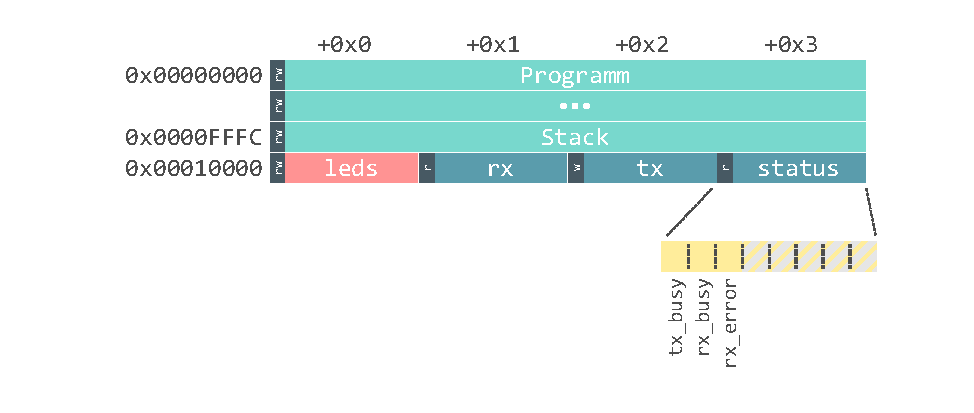
\includegraphics[scale=1]{img/memory.pdf}
            \caption{Speicher mit IO Bereich}
            \label{fig:io}
        \end{figure}

        \lstinputlisting[style=VHDL,caption={Adressaufteilung im Speicher},linerange={56-70},label=lst:memory]{../../CPU/Design/src/memory/memory.vhd}
        \newpage
        \lstinputlisting[style=VHDL,caption={Leseprozess für die Peripherie},linerange={39-47},label=lst:peripherie-read]{../../CPU/Design/src/io/peripherie.vhd}
        \lstinputlisting[style=VHDL,caption={Schreibeprozess für die Peripherie},linerange={50-63},label=lst:peripherie-write]{../../CPU/Design/src/io/peripherie.vhd}

        \subsection{LED}
            Es stehen acht LED's auf dem \textit{FPGA}-Board zur Verfügung die über den erweiterten Speicherbereich
            angesteuert werden können. Der Status der LED's kann hierbei gesetzt sowie abgefragt werden.
            Dazu dienen die beiden Prozesse in \textit{peripherie.vhd} (Siehe Listing \ref{lst:peripherie-read} und \ref{lst:peripherie-write}).

        \subsection{UART}
            Zusätzlich steht eine \textit{UART}-Schnittstelle zu Verfügung die es erlaubt Byteweise Daten
            zu senden oder empfangen.
            Dabei wurde das Modul im Rahmen dieser Arbeit nicht entwickelt und ist somit ein Fremdmodul \cite{vhdl-uart}.
            Es funktioniert jedoch nach dem gleichen Prinzip des \textit{Memory-Mappings}.
            Wie Listing \ref{lst:peripherie-read} und \ref{lst:peripherie-write} zeigen,
            besteht es aus drei Adressbereichen (Status, RX und TX) aus denen gelesen bzw. in die geschrieben werden kann.
            


\newpage
\listoffigures
%\lstlistoflistings
\printbibliography

\end{document}